\documentclass{article}
% Margin definition.
\usepackage[a4paper,total={6.8in, 8.5in}]{geometry}
\usepackage{parskip}
% Images.
\usepackage{graphicx}
\usepackage[hidelinks, bookmarks=true]{hyperref}
\usepackage{float}
% Encoding.
\usepackage[english]{babel}
\usepackage[utf8]{inputenc}
% Allow multiline comments
\usepackage{verbatim} 
% Helvetic font.
\usepackage[scaled]{helvet}
\renewcommand\familydefault{\sfdefault} 
% Header for UA logo.
\usepackage{fancyhdr}
% Dots in index.
\usepackage[titles]{tocloft}
\renewcommand{\cftsubsecleader}{\Large\cftdotfill{0}}
\renewcommand{\cftsecleader}{\Large\cftdotfill{0}}
\renewcommand{\cftsecfont}{\large\bfseries\scshape}
\renewcommand{\cftsubsecfont}{\scshape}
\renewcommand*{\HyperDestNameFilter}[1]{\jobname-#1}
% Dot after number in (sub)sections and in toc.
\renewcommand{\cftsecaftersnum}{.}
\renewcommand{\cftsubsecaftersnum}{.}
\usepackage{titlesec}
\titlelabel{\hspace{-0.5cm}\quad}
\usepackage[letterspace=45]{microtype}
\newcommand*{\fullref}[1]{\hyperref[{#1}]{\autoref*{#1} \nameref*{#1}}}
% Header with UA logo definition. 
\pagestyle{fancy}
\fancyhf{}
\chead{
    
\includegraphics[width=5in]{./images/header_ua.png}
}
\setlength\headheight{20pt}
% Footer with page number.
\rfoot{Page \thepage}
\renewcommand{\footrulewidth}{0.1pt}
% Rename table of contents title to "Index"
\renewcommand{\contentsname}{\normalsize Index \vspace{0.6cm}}
% Add text with hyperlink
\usepackage{hyperref}
%\hypersetup{
%    colorlinks=true,
%    linkcolor=blue,
%    filecolor=magenta
%}
% Water mark
\newsavebox\mybox
\usepackage[printwatermark]{xwatermark}
\usepackage{xcolor}
\usepackage{tikz}
% paragraph
\newcommand\tab[1][1cm]{\hspace*{#1}}
\setlength\parindent{24pt}
%images
 \usepackage{graphicx}
\usepackage{caption}
% footnotes at bottom
\usepackage[bottom]{footmisc}
% Urls with line break
\usepackage{pdflscape}
% Drawing functions
\usepackage{tikz}
\usepackage{pgfplots}
\pgfplotsset{width=7cm, height=4cm, compat=1.17}

\usepackage{multicol}
\setlength{\columnsep}{1cm}

%%%%%%%%%%%% References/Bibliography %%%%%%%%%%%%
\usepackage{biblatex}
\addbibresource{bibliography.bib}

%%%%%%%%%%%%%%%%%%%%%%%%%%%%%%%%%%%%%%%%%%%%%%%%%

\begin{document}

%%%%%%%%%%%%%%%%%% Cover Page %%%%%%%%%%%%%%%%%%
\title{\vspace{-0.9cm}
       \vspace{1cm}
       \normalsize
       \raggedright\textbf{Title: \hspace{1.5cm} Anatomy of a Web Connection: A Brief Analysis} \\ \vspace{0.4cm}
       \raggedright\textbf{Autor: \hspace{1.3cm} Eduardo Santos} \\ \vspace{0.4cm}
       \raggedright\textbf{Date: \hspace{1.45cm} 21/03/2021} \\}
\author{}
\date{}

\maketitle
\thispagestyle{fancy}

%%%%%%%%%%%%%%%%%% END Cover Page %%%%%%%%%%%%%%%%%%

\vspace{-1.4cm}

\tableofcontents


\fontsize{10pt}{13pt}
\selectfont
\lsstyle

\titlelabel{\thetitle.\quad}	

\newpage

\section{Introductory Note}

\tab This assignment consists in the use of the \textit{traceroute} command followed by the domain ""www.cmu.edu"", and interpreting the results obtained.  

\noindent The specific objectives of this assignment are the following:

\begin{itemize}
    \item Identify the technologies, processes, actors and business models involved in an web connection;
    \item Identify possible social and economic implications associated with the points above mentioned.
\end{itemize}

\section{Summary / Abstract}

\tab This assignment is related to what can happen during a web connection.

Using the \textit{traceroute} command, we will be able to analyze how a web connection works, and the path that the packages take in that connection.
From that analysis, we will be able to reach a conclusion about the previously referred paths, and the hops of the connection, referring also the players involved in each hop.

This assignment will also contemplate some other points, such as the operations, processes, techniques and technologies involved in each step, trying to situate these in the framework of the ISO OSI model, as well as some possible social and economic implications triggered by the point previously mentioned.

\section{Framework}

The web as a major importance in our lives, without it, most of our daily common tasks, tasks that we consider easy, wouldn't be so easy as we wished to. 

We can find an entire "world" inside our computers, smartphones, etc. This is only possible because there are many technologies, processes and actors involved, all of them through an abstract layer that hides the real complexity of the whole system. The operations inside that layer might have significant social and economic implications.

\section{Web connection: Protocols/Mechanisms involved}

\tab In an Internet connection, there are 2 main participants: clients and servers.

Clients are devices that are connected to the Internet, they can be computers, smartphones, etc. Servers are also devices (specifically computers), they can store webpages, sites or apps. 
When a client makes a request to access a specific webpage, the server responds with a copy of the webpage, which is downloaded to the client's machine. This copy is then displayed in the user's web browser.

This is how a web connection works, at least at a very high-level. But there are many other parts involved in the connection. We will see a brief explanation of some of the mechanisms used during this connection.

\newpage

\subsection{Web browser}

\tab A web browser is a software application. That application is used for accessing the WWW\footnote{World Wide Web}. When a user makes a request for a web page, the web browser responds with the content from a web server, displaying the same content on the user's device/machine. That content is transferred using the HTTP\footnote{Hypertext Transfer Protocol}, which defines how many types of media are transmitted through machines on the web. We will address this protocol later on.

Websites save information about its users in files, those files are called cookies. They are stored in our computers for the next time we visit that website. For example, when we choose the option to store our username/email and password, that is made possible with the usage of cookies.

A web browser should not be confused with a search engine, the last one being a website that contains links to other websites.

\begin{figure}[H]
    \begin{center}
        
\includegraphics[width=0.3 \textwidth]{images/browsers.png}
        \caption{\href{https://www.google.com/url?sa=i&url=https\%3A\%2F\%2Fventurebeat.com\%2F2020\%2F01\%2F15\%2Fbrowser-benchmark-battle-january-2020-chrome-firefox-edge-brave\%2F&psig=AOvVaw1kepSAmHxWnyx7E\_xnjq2a&ust=1617098633832000&source=images&cd=vfe&ved=0CAIQjRxqFwoTCJjgy\_-f1e8CFQAAAAAdAAAAABAD}{\underline{Some of the most used browsers at the moment}}}
    \end{center}
\end{figure}

\subsection{TCP/IP}

\tab TCP\footnote{Transmission Control Protocol} and IP\footnote{Internet Protocol} are often referred together as TCP/IP, an Internet protocol suite. This suite is a set of communications protocols, establishing how data should be packetized, addressed, transmitted, routed, and received in an end-to-end data communication.

Architecturally speaking, TCP/IP can be divided into a four-layer model, which consists in the following layers:

\begin{itemize}
    \item \textbf{Application layer} - In this layer, applications/processes create user data, communicating this to other applications. This can be done on the same host, or on a different one;
    \item \textbf{Transport layer} - performs host-to-host communications, this communications can be on the local network, as well as on remote networks (separated by routers);
    \item \textbf{Internet layer} - provides a uniform networking interface, hiding the actual topology of the underlying network connections;
    \item \textbf{Link layer} - defines the networking methods in the local network link on which hosts communicate, this is done without routers.
\end{itemize}

\newpage

\subsection{DNS} 

\tab DNS\footnote{Domain Name System} is a naming system for computers, services, or other resources connected to the Internet, although it can also be done in a private network.

The way that humans access information online is through domain names, unlike web browsers, that interact through IP addresses. DNS job is to translate these domain names to IP addresses.

We've seen that web browsers communicate through IP addresses, but what is an IP address?

An IP address is an unique address that identifies a device on the Internet or a local network. Using this address, machines can find each other on that network.

\begin{figure}[H]
    \begin{center}
        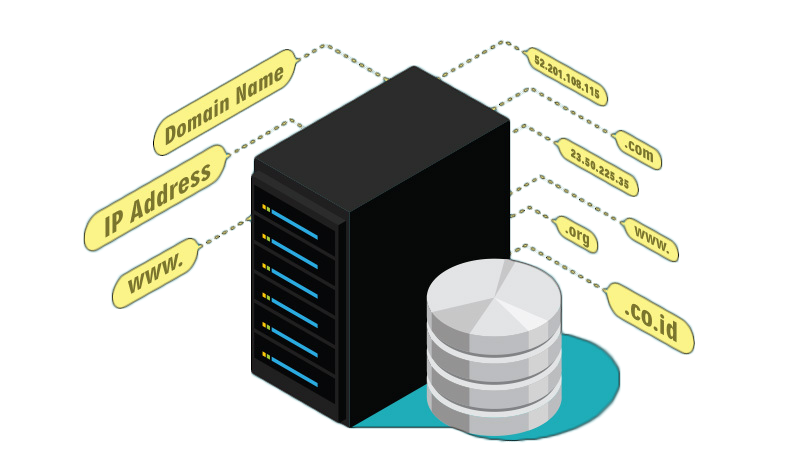
\includegraphics[width=0.6 \textwidth]{images/dns.png}
        \caption{\href{https://www.google.com/url?sa=i&url=https\%3A\%2F\%2Fwww.pcmag.com\%2Fhow-to\%2Fhow-and-why-to-change-your-dns-server&psig=AOvVaw0kvZbAUtDVX3KBUpHmIdu4&ust=1617099982879000&source=images&cd=vfe&ved=0CAIQjRxqFwoTCPCEmYOl1e8CFQAAAAAdAAAAABAD}{\underline{DNS}}}
    \end{center}
\end{figure}

\subsection{HTTP}

\tab HTTP is an application-layer protocol used when transmitting hypermedia documents (such as HTML\footnote{Hypertext Markup Language}). Its main purpose is to provide communications between web browsers and web servers, although it can be used for other ones. 

This protocol follows a client-server model: a client opens a connection and makes a request, then waits to receive the response. Being a stateless protocol, the server doesn't store any data between two requests.

\section{What is the \textit{traceroute} command?}

\tab Traceroute is a network diagnostic tool used for real-time tracking of the path taken by a packet on an IP network, from the beginning till the end. This tool also reports the IP addresses of all the routers that are on its path, showing also the time taken for each hop made by the packet during its route.

Traceroute normally uses ICMP\footnote{Internet Control Message Protocol} echo packets with a TTL\footnote{Time To Live} that varies. For accuracy aspects, each hop is (usually) queried three times, to better measure the response. 

\newpage

\subsection{Executing the command}

\tab Executing the command \textit{traceroute -I www.cmu.edu}, we obtain the following output:

%Added [H] after so that image is placed after the text above
%This is only possible by adding also \usepackage{float} to the preamble
\begin{figure}[H]
    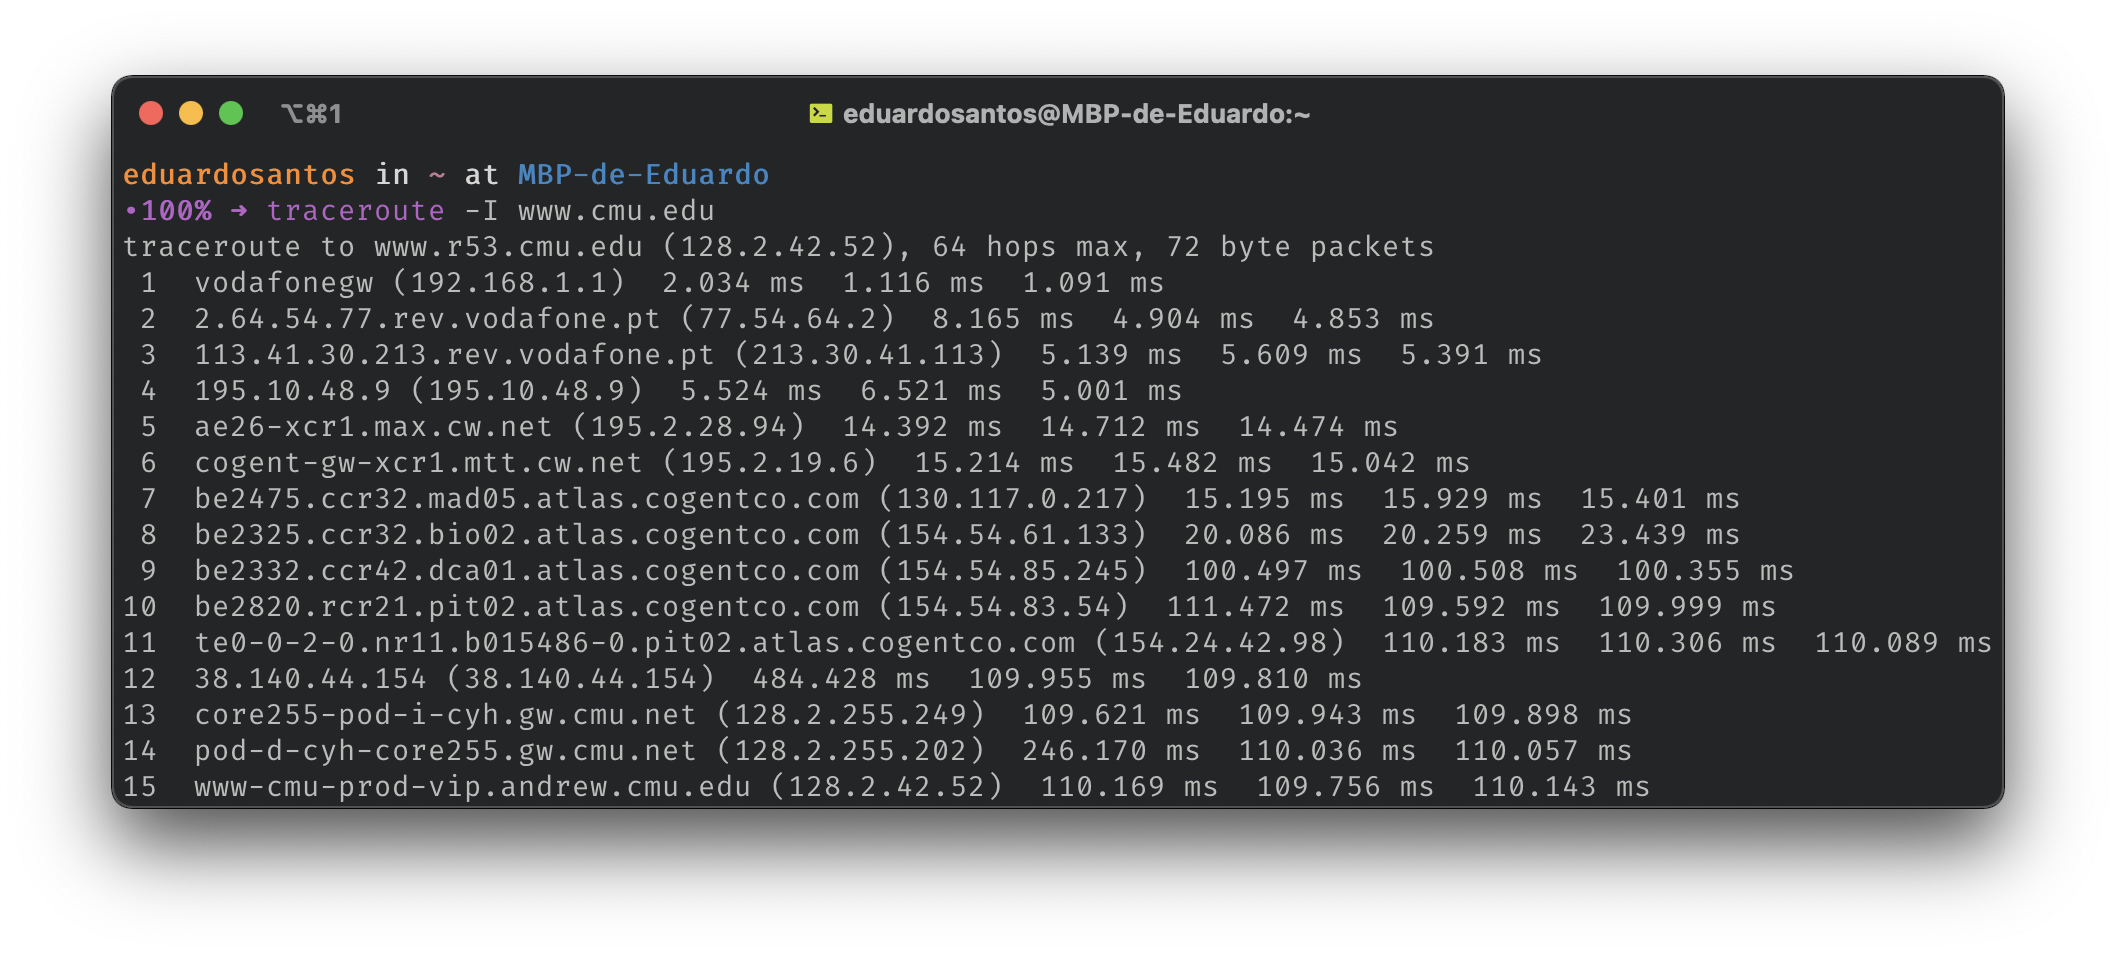
\includegraphics[width=1 \textwidth]{images/tracerouteHome.png}
    \caption{Output of the \textit{traceroute} command, executed inside home network, on 29/03/2021, at 19h27}
\end{figure}

\begin{figure}[H]
    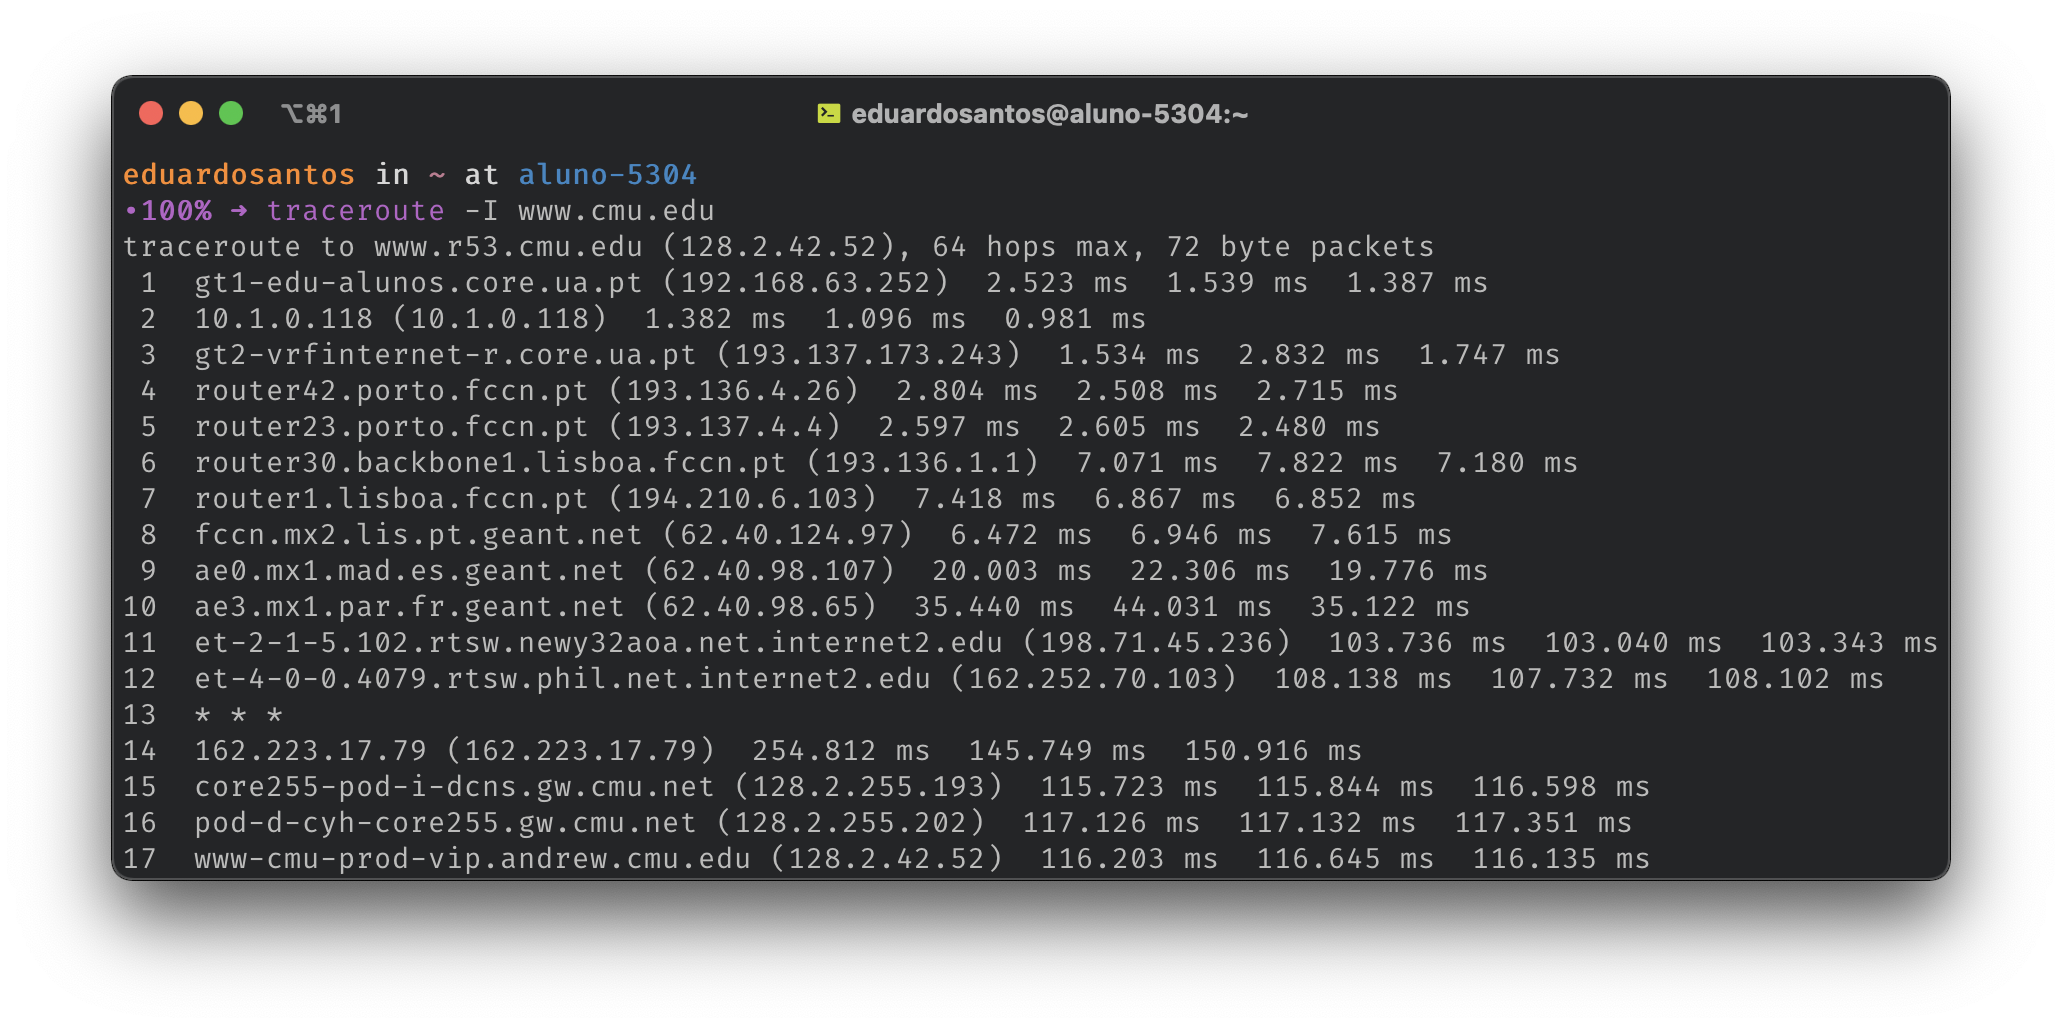
\includegraphics[width=1 \textwidth]{images/tracerouteUA.png}
    \caption{Output of the \textit{traceroute} command, executed inside University of Aveiro's network, on 26/03/2021, at 15h12}
    \label{tracerouteUA}
\end{figure}


The \textit{-I} parameter was used because, instead UDP\footnote{User Datagram Protocol}, what we wanted is to use ICMP echo, to prevent getting too many "Request Timed Out" messages. 

The ICMP echo requests and the ICMP echo reply messages are commonly known as ping messages. Ping is a computer network administration software utility and is used to test if a host is reachable on an IP network. This utility works by sending this ICMP echo request packets to the target host, waiting for it to reply through an ICMP echo reply.

\subsection{Interpretation of the executed command's results}

\vspace*{\fill}
    \begin{center}
        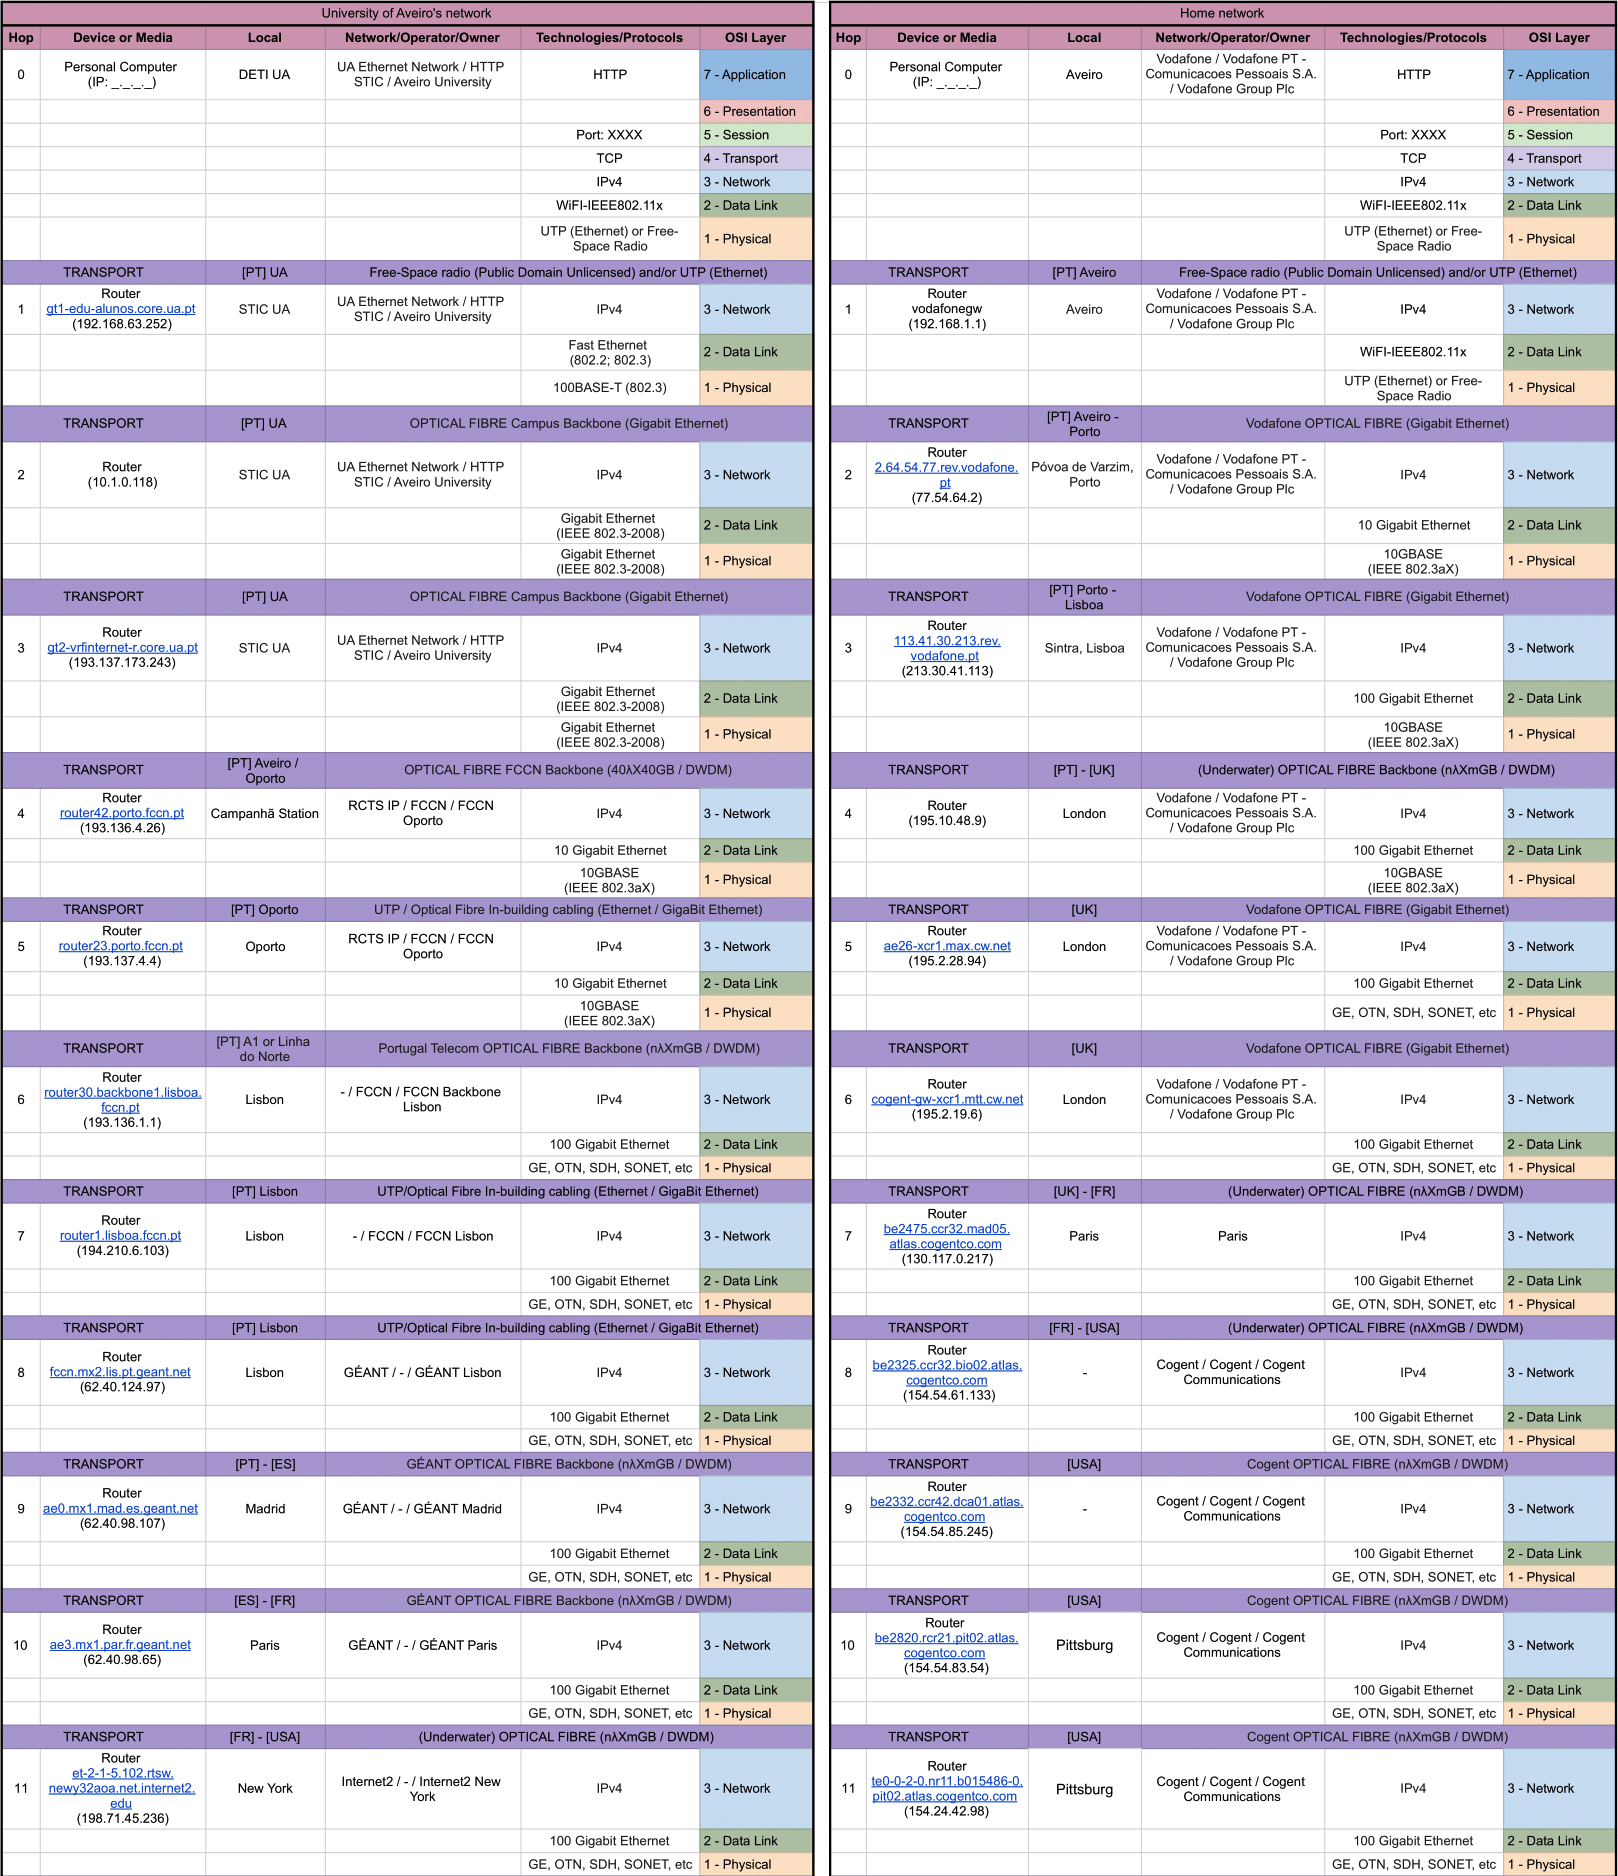
\includegraphics[width=1 \textwidth]{images/traceroute_part1.png}
    \end{center}
\vspace*{\fill}

\vspace*{\fill}
    \begin{figure}
        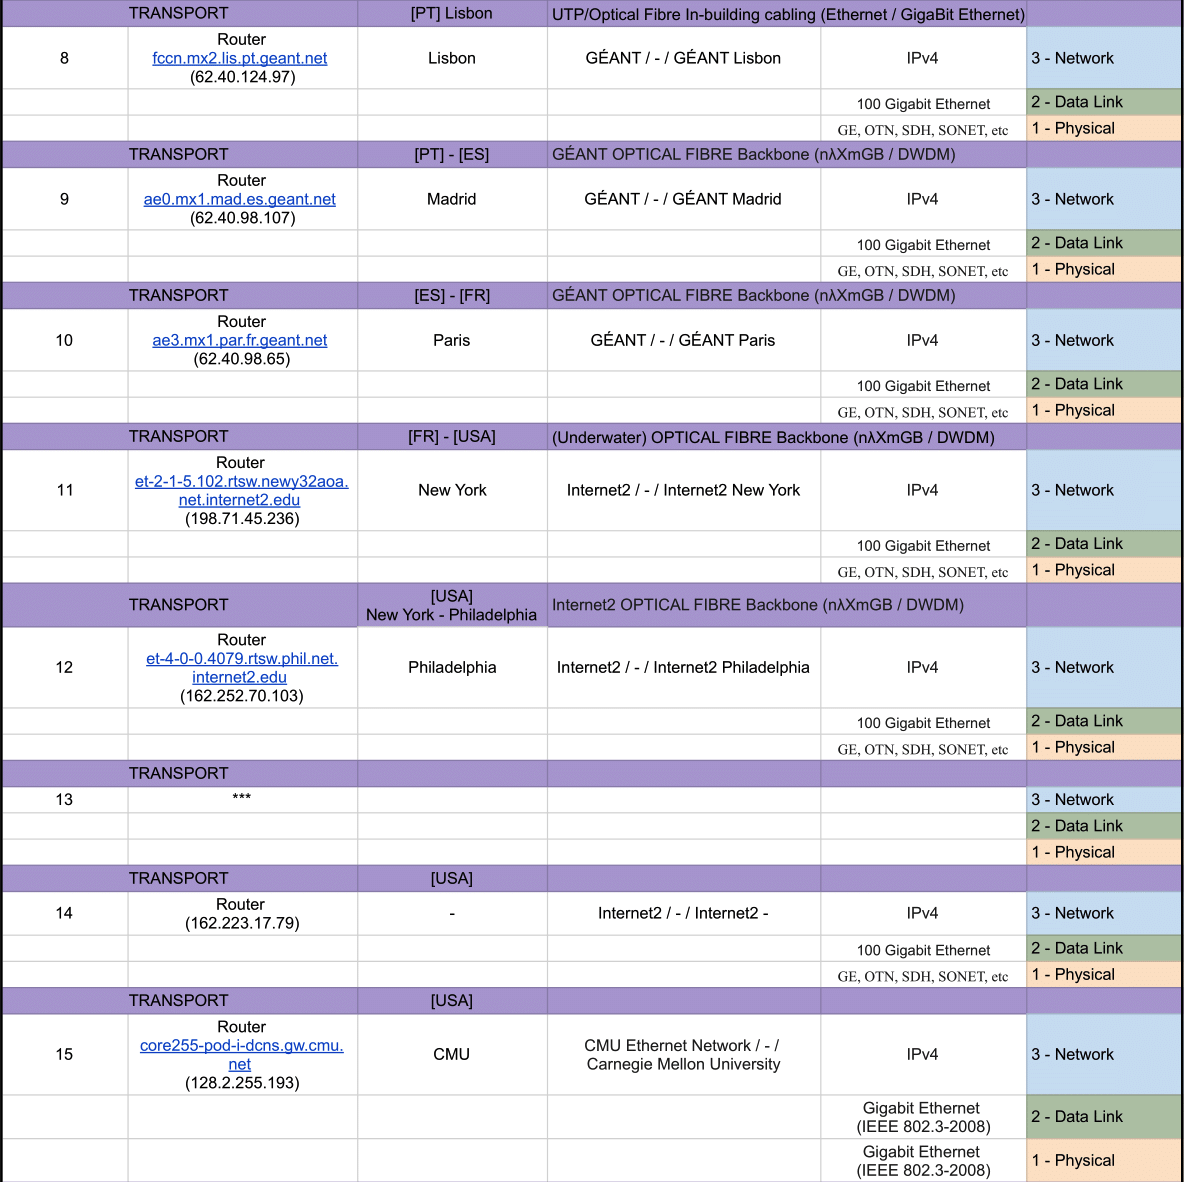
\includegraphics[width=1 \textwidth]{images/traceroute_part2.png}
        \caption{Table containing details of the \textit{traceroute} command paths, for both University of Aveiro and home networks}
    \end{figure}
\vspace*{\fill}

\subsubsection{Identifying the local of each IP address}

\tab To identify the local of an IP address, a tool called \textit{IP Tracker} was used. This tool, which can be accessed through the web, tracks/traces a given IP address, retrieving all possible information about it (region, city, postal address, etc.).

Although this information is quite accurate, sometimes it's not possible to get any data about a specific IP, this can happen due to many reasons, but normally is because of security ones.

\subsubsection{"*** Request timed out" hops}

\tab If we look at the Figure \underline{\ref{tracerouteUA}}, we can see that, on hop 13, there was a "Request timed out", this probably happened because some routers won't answer to ICMP requests, and this is made on purpose. If we could see all the routers, the path could be compromised, because there may be some key routers on the connection, and, if attacked, those situations could cause serious security problems on the path.

A possible attack could be, for example, an ICMP flood DDoS\footnote{Distributed Denial-of-Service} attack, commonly referred as Ping flood attack. This is a DoS\footnote{Denial-of-Service} attack in which a large number of ICMP echo requests (pings) are sent to a specific device by an attacker, with the intention of overwhelming it. 

By flooding the device with this packages, it becomes unapproachable to normal traffic. Being distributed, it means that the attacks to a target come from multiple devices.

\subsubsection{Logs variation during time}

\tab For each location (University of Aveiro and my home), there were executed multiple \textit{traceroute} commands. Analysing the obtained results, there are some differences between logs from the same network, when executed at different times. 

This difference can be because, at a specific time, specific path can have a lot of load due to a large number of requests. This will significantly increase the latency of the entire connection, which is something to avoid.

To avoid this situation, new requests are sent through other routers, in a way that makes the connection as efficient as possible.

\newpage

\section{Social/Economic implications}

\tab The Internet has undoubtedly brought a window to the entire world, all through a computer screen, and the fact that such a small window can display so much information is surprising.

None of this would be possible without the technologies mentioned above. These have changed the way we look at the world, and have shown us that knowledge has no end. And we cannot just refer to knowledge, there are a multitude of aspects that the Internet has brought us, and ease of communication is another very important one.

Another thing to mention is the amount of technologies, processes, actors and business models that are involved in a "simple" connection to a given domain, as in this case the CMU\footnote{Carnegie Mellon University}.

From this large number of participants, we can conclude that there are many aspects that can affect a connection, from physical aspects - connection problems, problems with routers - to aspects more related to the economic/social part - network companies and their ups and lows in the market, social crises that can lead to a greater load on the network, etc.

Due to the COVID-19 global pandemic, in the last year we have felt these same economic and social changes and how much this can affect, in this case, the Internet and its stakeholders. Due to the massive number of people who are forced to stay at home, to all jobs that were once in a enterprise environment and are now from home, among other aspects, the Internet has suffered a huge load of requests-responses, something that clearly has its repercussions.

Because of this significant increase in the load of the web, the players involved in the connections, in this case the network companies, had to take steps to scale their services, so that the world would not stop, at least due to the lack of this precious resource, that is the Internet.

\section{Conclusion}

\tab With this assigment, we were able to see the path that taken by a connection to the domain "www.cmu.edu", and covered many other aspects that are present in it, like the technologies, processes, actors and business models.

We could also get an overview of how some technologies/tools involved in a web connections work. 

To conclude, we made an assumptions of social and economic implications that can affect an entire connection.

\newpage

% Add "References" to table of contents
\addcontentsline{toc}{section}{References}
% No cite makes all references appear, even if there's no citation on the text
\nocite{*}
\printbibliography

\end{document}